\newpage
\chapter{Introducción}

En 2020, el \textbf{cáncer de próstata, (Prostate Cancer, PCa)} fue el segundo tipo de cáncer más frecuente, y el quinto más mortal, en varones \cite{GlobalCancer}. Una \textbf{biopsia de próstata} es una prueba que consiste en la extracción de pequeños tejidos de la próstata para examinar posibles signos de cáncer (Ver Figura \ref{fig:biopsias_ejemplos}). El \textbf{Sistema de Puntuación de Gleason (Gleason Score)} es una calificación, en el rango de 2 a 10, que se da a biopsias de la próstata tras ser examinadas bajo un microscopio \cite{GleasonGov}. Valores más altos indican cánceres más agresivos y de crecimiento más rápido. En 2014 la \textbf{Sociedad Internacional de Patología Urológica (International Society of Urological Pathology, ISUP)} propuso un nuevo sistema basado en la Puntuación de Gleason, que propone cinco grupos ordenados (\textbf{Gleason Groups, GGs}) \cite{ISUP2014Disc}:
\begin{itemize}
\item \textbf{GG1: } Cáncer de grado bajo. Puntuación de gleason 6 o inferior.
\item \textbf{GG2: } Cáncer de grado medio. Puntuación de gleason 7.
\item \textbf{GG3: } Cáncer de grado medio pero más agresivo que GG2. Puntuación de gleason 7 pero percibido más agresivo.
\item \textbf{GG4: } Cáncer de grado alto. Puntuación de gleason 8.
\item \textbf{GG5: } Cáncer de grado alto. Puntuación de gleason 9 o 10.
\end{itemize}

\begin{figure}[H]
    \centering
    \begin{subfigure}[b]{0.3\textwidth}
        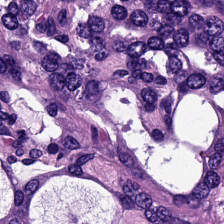
\includegraphics[width=\linewidth]{images/EjemploBiopsia1.png}
    \end{subfigure}
    \hfill
    \begin{subfigure}[b]{0.3\textwidth}
        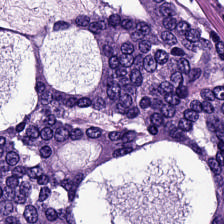
\includegraphics[width=\linewidth]{images/EjemploBiopsia2.png}
    \end{subfigure}    
    \hfill
    \begin{subfigure}[b]{0.3\textwidth}
        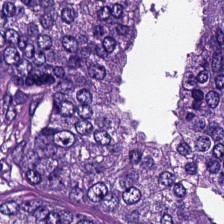
\includegraphics[width=\linewidth]{images/EjemploBiopsia3.png}
    \end{subfigure}

    \caption{Tres imágenes correspondientes a tres biopsias distintas.}
    \label{fig:biopsias_ejemplos}
\end{figure}


En el campo de la \textbf{Inteligencia Artificial (IA)}, la necesidad de asegurar transparencia y confiabilidad a dado pie a acuñar el término de \textbf{Inteligencia Artificial eXplicable (eXplainable Artificial Inteligence, XAI)} \cite{XAIManifesto}. El uso de XAI es especiamente importantes en ámbitos donde la toma de decisiones repercute directamente en la vida de las personas, como es el caso de la medicina. La Unión Europea ha propuesto una \href{https://eur-lex.europa.eu/eli/reg/2024/1689/oj}{regulación} para el uso de IA asistida en estos aspectos, entre ellos, que estos sistemas sean capaces de explicar sus decisiones de forma clara y comprensible.

Dentro del campo de la XAI, hay diferentes propuestas para la evaluación y la mejora de las explicaciones generadas. Por un lado, herramientas como \textbf{REVEL} \cite{REVEL} permiten analizar la calidad de las mismas de manera robusta. Por otro, enfoques como \textbf{X-SHIELD} \cite{XSHIELD} buscan mejorar las explicaciones mediante técnicas de regularización que aseguran el buen comportamiento de la generación de explicaciones. Aplicar estas técnicas en imagen médica puede ayudar a mejorar la interpretación de las personas profesionales de la salud de las decisiones de una IA que asista.

En este contexto este Trabajo de Fin de Máster trata de resolver el problema de \textbf{construir un modelo de IA de clasificación para lesiones cancerosas en biposias de próstata} y de la \textbf{mejora en interpretabilidad del modelo mediante técnicas de XAI}. Para esto se vamos a utilizar las herramientas REVEL y XSHIELD, y propondremos posibles mejoras de XSHIELD.


El TFM se estructura del siguiente modo. En primer lugar vamos a introducir los fundamentos teóricos necesarios para el correcto entendimiento del trabajo realizado (Capítulo \ref{cap:ft}). Después se va a hacer un estudio del estado del arte (Capítulo \ref{cap:eda}). A continuación presentamos las propuestas de este TFM (Capítulo \ref{cap:met}). En el Capítulo \ref{cap:exp} se describe el conjunto de datos con el que trabajamos, los distintos experimentos que realizamos y discutimos los resultados . Finalmente en el Capítulo \ref{cap:conc} se incluyen conclusiones y posibles trabajos futuros.


\section{Objetivos}

El objetivo principal del TFM es la utilización (y propuesta) de técnicas de evaluación y mejora de explicaciones  para modelos de clasificación de imágenes para detección de tejidos cancerosos en biopsias de próstata. Para el desarrollo del TFM, se divide el objetivo en distintos subobjetivos:

\begin{itemize}
\item Revisión del estado del arte \highlight{Cuál?}.
\item Estudio del código que implementa \cite{REVEL, XSHIELD} para su correcto entendimiento.
\item Proposición de nuevos métodos XAI para mejora de explicaciones para modelos de explicación.
\item Modificación del código para implementar dichas propuestas.
\item Diseño de los experimentos a realizar e implementación de estos.
\item Evaluación de los resultados y subsecuente discusión.
\end{itemize}

Aquí introduciría el objetivo principal del TFM y lo dividiría en algunos sub-objetivos (revisión del estado del arte, estudio de las implementaciones de las métricas ReVEL/regularización X-Shield, proposición de mis regularizaciones, implementación de estas, experimentación y finalmente evaluación/discusión de estos). 


\section{Planificación}

\highlight{
En esta sección hablo de cómo me he planificado el proyecto según estudio del problema/diseño de mis modelos/implementación/experimentación (haría una tabla). Luego haría una comparación de mi planificación vs cómo se ha repartido finalmente y haría una estimación final de cuántas horas me ha llevado el TFM y en cuánto se estima el coste del proyecto final.

POR HACER
}


\clearpage
\chapter{Fundamentos teóricos} \label{cap:ft}
\highlight{
Finalmente tendría la sección más relevante para este TFM que sería la de . Primero haría una introducción más general basándome en este paper (https://www.sciencedirect.com/science/article/pii/S1566253523001148) y luego explicaría LIME para explicar bien lo que son las métricas REVEL y XSHIELD más adelante.} 


\section{Aprendizaje automático}

El \textbf{aprendizaje automático} (AA) o \textbf{machine learning} (ML) es una rama de la \textbf{inteligencia artificial} que se encarga del desarrollo de algoritmos que aprendan de datos o experiencias con el fin de mejorar su rendimiento en ciertas tareas \cite{alpaydin_introduction_2010-1, Mostafa2012, PatternRecogLibro, pml1Book}. Estos algoritmos disponen de un \textbf{modelo} definido por ciertos parámetros y dichos parámetros serán los que se aprendan a través del \textbf{entrenamiento} o \textbf{aprendizaje}.

Para saber a qué nos referimos cuando se habla de que el algoritmo \textit{``aprende''} conviene destacar la siguiente definición proveniente de \cite{mitchell_machine_1997}: \textit{``Un programa se dice que aprende de una experiencia E con respecto a una clase de tareas T y a una medida de rendimiento T, si su rendimiento en las tareas en T, medido por P, mejora con la experiencia E."}

El AA se utiliza habitualmente para resolver problemas complejos que no se pueden o se saben resolver con algoritmos tradicionales diseñados por humanos. Además se requiere tener datos de los que poder aprender. Algunos de los campos donde se utilizan el AA para resolver este tipo de problemas son el procesamiento de lenguaje natural, el reconocimiento del habla o la visión por computador, entre muchos otros.

Los algoritmos de AA se clasifican en distintos paradigmas dependiendo de los datos o experiencia de la que se disponga. Existen tres paradigmas principales: el \textbf{aprendizaje supervisado}, el \textbf{aprendizaje no supervisado} y el \textbf{aprendizaje por refuerzo} \cite{Mostafa2012,Goodfellow-et-al-2016}.

El aprendizaje supervisado hace referencia a los algoritmos de AA en los que se tiene un conjunto de datos agrupados en pares dato-\textbf{etiqueta}. La etiqueta se corresponde con la salida que se requiere del algoritmo de AA cuando tenga de entrada dicho dato. Un ejemplo típico de conjunto de datos de este tipo sería un conjunto de imágenes de números escritos a mano y para cada imagen el número que está escrito en dicha imagen.

El aprendizaje no supervisado hace referencia a los algoritmos de AA en los que se disponen de datos que no están etiquetados. En este tipo de algoritmos no se quiere aprender algo específico de los datos sino más bien encontrar patrones o estructurar los datos de entrada. Por ejemplo se dispone de distinta información relativa a libros (autor, título, número de páginas, etc) y el algoritmo categoriza los libros en distintas categorías, aunque no se sepa a qué se corresponde cada categoría.

En el aprendizaje por refuerzo no se disponen de datos de entrada, sino de una entrada y una \textit{recompensa} correspondiente a cada salida posible para dicha entrada. Este tipo de AA es especialmente útil para aprendizaje de juegos o tareas relacionadas con la teoría de control.

Para este TFG es relevante el aprendizaje supervisado. En particular serán relevantes los dos siguientes problemas típicos de aprendizaje supervisado.

\subsection{Problema de clasificación}
Este problema trata de clasificar las entradas de un tipo concreto en un número de clases $k$. Es decir, para una entrada el programa deberá clasificar dicha entrada en una de las $k$ clases. Por lo tanto el algoritmo produce una función $f:\mathbb{R}^n \rightarrow \{1,...,k\}$ que a cada entrada $\bx$ le asocie una clase $y = f(\bx)$. Dicha función tratará de aproximar una función objetivo $g$ que clasifique perfectamente todas las entradas.

Para este problema se disponen de una serie de datos de entrada $\{\bx_1,...,\bx_N\}$ con $\bx_i\in\mathbb{R}^n$ y sus clases correspondientes $\{y_1,...,y_N\}$ con $y_i \in \{1,...,k\}$. 

Algunas formas de resolver estos problemas son mediante árboles de clasificación, máquinas de vectores-soporte o mediante redes neuronales.

Un caso particular de este problema que es más relevante para este trabajo es el caso en el que hay dos clases. Este problema se denomina \textbf{problema de clasificación binaria}. En este TFG se tratará de determinar visibilidad de puntos de la cara de una persona en una imagen luego las dos clases se corresponden con visible o no visible.

\subsection{Problema de regresión}
Este problema es similar al de clasificación, pero la función que aprende el algoritmo es de la forma $f:\mathbb{R}^n \rightarrow\mathbb{R}^m$. Por lo tanto ahora el programa debe predecir un valor numérico (o varios si $m > 1$) para una entrada concreta. Al igual que ocurría en el problema de clasificación se disponen de una serie de datos de entrada y el resultado que se espera del programa para dichas entradas, es decir $\{\bx_1,...,\bx_N\}$ con $\bx_i\in\mathbb{R}^n$ y  $\{\by_1,...,\by_N\}$ con $\by_i \in \mathbb{R}^m$. 

Algunas formas de resolver este tipo de problemas son mediante la regresión lineal, máquinas de vectores-soporte o redes neuronales.

\subsection{Optimización} \label{optimización}

Ya se ha hablado de algunos problemas de AA. En ellos se quiere mejorar el rendimiento de una función $f$ para una tarea. La forma en la que se mide el rendimiento es mediante otra función denominada \textbf{función de error}, \textbf{función de pérdida} o \textbf{función de coste} \cite{Goodfellow-et-al-2016}. Esta función mide el error de la aproximación de la salida de $f$ para una entrada $\bx$. Por lo tanto se busca minimizar dicha función.

Por ejemplo, una función de coste habitual es el error cuadrático medio:

\begin{align*}
ECM = \frac{1}{n}\sum_{i=1}^{n}(y_i-\hat{y_i})^2
\end{align*} 

Donde $\hat{y_i}$ es la predicción de nuestro modelo para un dato $x_i$ y $y_i$ es el valor correcto de salida para esa entrada.

El método principal en el AA para minimizar dicha función es el \textbf{gradiente descendente}. Este método iterativo se basa en que, para una función multivariable dos veces diferenciable, el gradiente de dicha función en ese punto (que es un vector) apunta en la dirección contraria al ascenso más empinado. Por lo tanto tomando pasos en la dirección contraria al gradiente, debería disminuir la función de coste y por lo tanto dar un mejor rendimiento.


Se recuerda que el gradiente de una función $E:\mathbb{R}^n \rightarrow \mathbb{R}$ en un punto no es más que le vector compuesto de las derivadas parciales respecto a cada variable en dicho punto:

\begin{align*}
\nabla E(\bw) = \left[ \frac{\partial E}{\partial x_1}(\bw),...,\frac{\partial E}{\partial x_n}(\bw) \right]^\top
\end{align*}


Normalmente, el método utilizado para resolver el problema de AA hace que las funciones que se pueden representar en la solución estén parametrizadas por un vector de parámetros o \textbf{pesos} $\bw$. Por ejemplo, en un problema de regresión con función objetivo $f:\mathbb{R}^n \rightarrow \mathbb{R}$ que se plantea resolver mediante regresión lineal se tiene que la función que se aprende toma la forma: 
\begin{align*}
f_\bw(\bx) = \bw^\top \bx \quad \quad , \bx \in \mathbb{R}^n, \bw \in \mathbb{R}^n
\end{align*}
 
Donde el vector $\bw$ son los parámetros que se pueden cambiar a la función para mejorar su rendimiento.

La función de coste dependerá de dichos parámetros. Luego el gradiente descendiente cambiará el valor de los parámetros en cada paso buscando minimizar la función de coste. Estos cambiarán según la siguiente regla:
\begin{align*}
\bw_n = \bw - \eta \nabla E(\bw)
\end{align*} 
Donde $\bw_n\in\mathbb{R}^l$ son los nuevos parámetros, $\bw\in\mathbb{R}^l$ son los parámetros del paso actual, $E$ es el función de coste, $\nabla E$ representa el gradiente de $E$ y $\eta$ es un hiperparámetro (parámetro del algoritmo) en $\mathbb{R}$ llamado \textbf{learning rate}(lr).

El lr determina el tamaño de los pasos tomados por el algoritmo en cada iteración. Un valor del lr alto puede hacer que	el algoritmo converja más rápido pero también puede hacer que el algoritmo no llegue a converger o se salte soluciones. Por otro lado un valor bajo del lr hace que el algoritmo converja demasiado lento a un mínimo de la función. En la práctica se suelen utilizar métodos que hacen que el lr varíe a lo largo del entrenamiento, normalmente de mayor a menor.

El algoritmo del gradiente descendente inicia los pesos $\bw$ a un valor aleatorio y empieza a iterar con la regla anteriormente descrita buscando reducir el error en cada paso durante un número de \textbf{épocas} (cada época itera sobre todos los datos de entrenamiento), aunque hay otros criterios de parada del algoritmo. En caso de ser satisfactorio el algoritmo para en un mínimo local (o global idealmente) del error de pérdida. 

El cálculo del gradiente del error conlleva utilizar todos los datos de entrenamiento lo que en la práctica resulta muy costoso. Por ello se suele utilizar el \textbf{descenso de gradiente estocástico} (SGD), que en cada paso calcula una estimación del gradiente real a partir de un subconjunto aleatorio de los datos de entrenamiento denominado \textbf{minibatch}. Destacar que los datos de entrenamiento no se deben repetir entre \textit{minibatches} hasta que se hayan utilizado todos los de entrenamiento entre cada repetición.

\subsection*{Sobreentrenamiento}

Cuando se optimiza un modelo, puede ocurrir que el modelo se ajuste muy bien para los datos de entrada con los que se ha entrenado, pero tenga mal rendimiento para datos con los que no se ha entrenado y por lo tanto no generaliza bien lo aprendido de los datos de entrenamiento al problema. Cuando esto ocurre se dice que el modelo se ha \textbf{sobreentrenado} o \textbf{sobreajustado}. Una forma de identificar este problema es guardándonos un número de datos con los que no se va a entrenar el modelo y comparar el error del modelo a lo largo del entrenamiento de los datos de entrenamiento con los que nos se han guardado. El sobreentrenamiento se puede observar cuando el error en los datos con los que no se entrena empieza a aumentar a medida que se sigue entrenando el modelo como se puede ver en la Figura \ref{fig:sobreentrenamiento}.


\begin{figure}[h]
\noindent
\makebox[\textwidth]{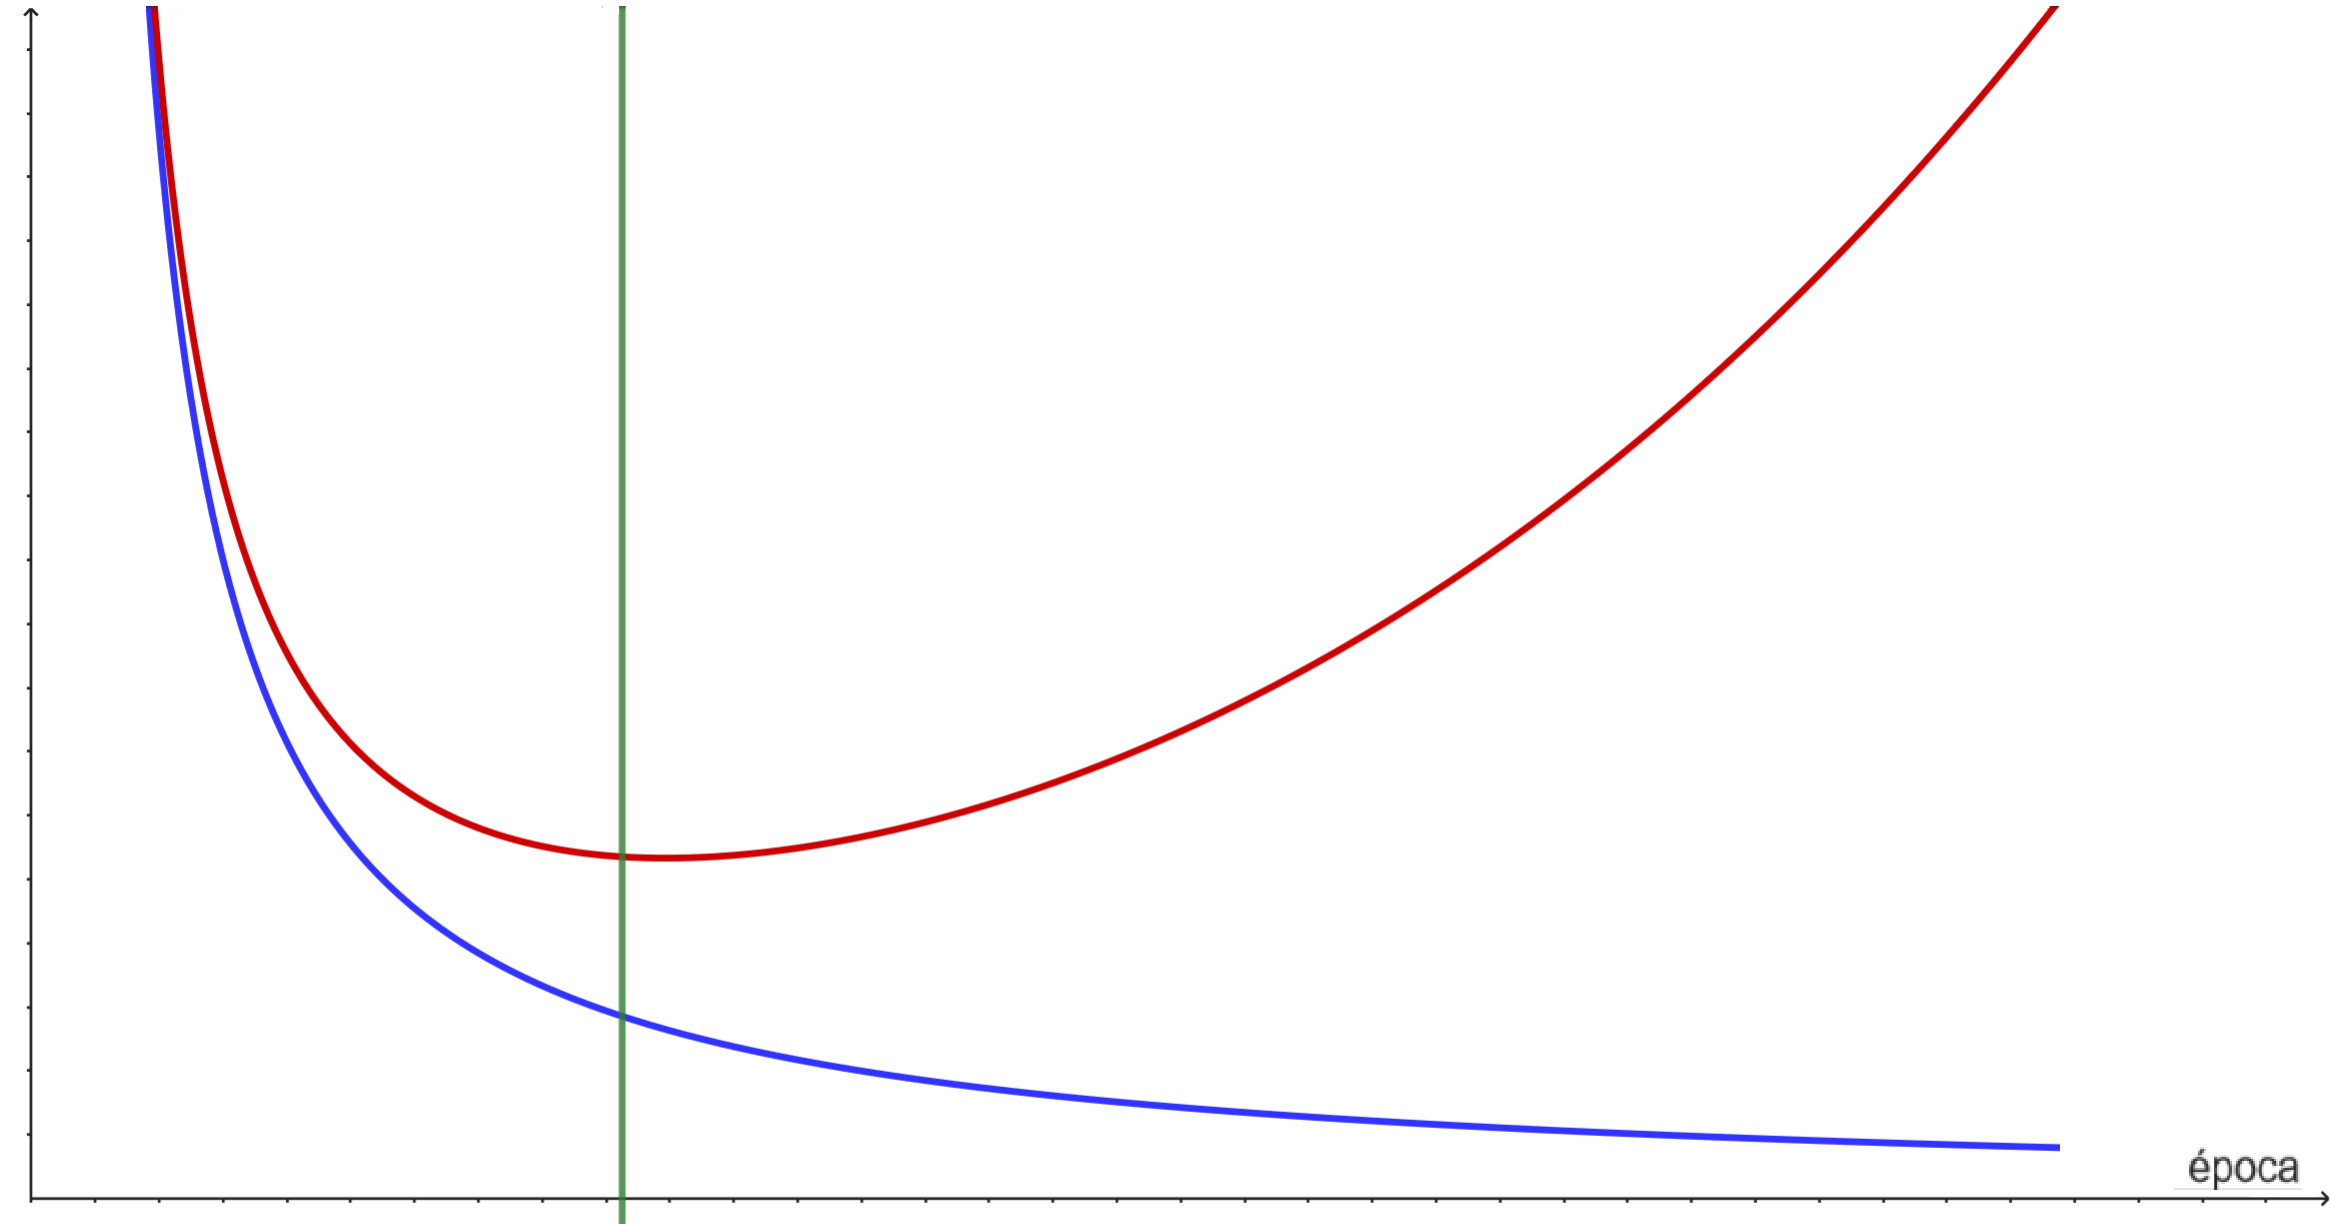
\includegraphics[scale=0.3]{images/sobreentrenamiento}}
\caption{ Esta figura muestra el error en entrenamiento en azul y el error en los datos con los que no se entrena el modelo en rojo a lo largo del entrenamiento. Se puede ver como a partir de la línea verde el modelo sigue aprendiendo de los datos de entrada pero empeora el poder de generalización con los datos con los que no entrena.}
\label{fig:sobreentrenamiento}
\end{figure}

\section{Deep Learning}
\textbf{Deep learning}(DL) \cite{DeepLearningFoundationsConcepts, Goodfellow-et-al-2016, LeCun-Yann-Bengio, UnderstandingDeepLearning, Schmidhuber_2015} es un subcampo del AA determinado por los métodos con los que aprende y tipo de datos con los que trata. Los algoritmos de DL pueden tratar datos poco estructurados como pueden ser imágenes o textos. Este tipo de algoritmos automatizan la extracción de características, es decir, determinan qué información de los datos es relevante para la resolución del problema. Esto elimina mucha de la intervención necesaria por los humanos a la hora de crear el algoritmo.

El DL en los últimos años ha supuesto un avance significativo en muchos campos en los que apenas se avanzaba con otras técnicas de IA como el reconocimiento del habla o el procesamiento de lenguaje natural.

\subsection*{Redes neuronales}
Una \textbf{red neuronal} (\textit{artificial neural network}, ANN) \cite{NNPatternRecogLibro,Haykin,NNTricks} es un modelo de AA que consiste en una red conectada de \textbf{nodos} o \textbf{neuronas}. Cada neurona recibe una serie de números reales (señales) de las neuronas conectadas a esta, hace una operación con dichos números que resulta en otro número real y lo manda a los nodos conectados a esta. 

La operación que realiza una neurona con $n\in\mathbb{N}$ entradas es la siguiente:

\begin{align} \label{eq:salida_neurona}
y = \sum_{i=1}^{n}\sigma({w_i x_i} + w_0) \quad \quad , w_i,x_i \in \mathbb{R}
\end{align}

Dónde $x_i$ son las entradas de la neurona, $w_i$ son los \textbf{pesos} de la neurona, en particular a $w_0$ se le denomina sesgo, y $\sigma$ es una función de los números reales a los números reales y se le denomina \textbf{función de activación} \cite{article_func_activacion}. Al conjunto de los pesos de todas las neuronas de una red se les denomina, naturalmente, \textbf{pesos de la red}. A través de la modificación de dichos pesos es como se entrenará a una red para realizar una tarea concreta.

Existen dos tipos de ANN según el flujo de la información dentro de la red. Nos centramos en el caso en el que este flujo es una única dirección, en cuyo caso se tiene una \textbf{red neuronal hacia delante} (\textit{feedforward neural network} o \textit{multilayer perceptron}, MLP).

Las MLP son el modelo fundamental del \textit{Deep Learning}. Estas están compuestas por distintas \textbf{capas}, cada una compuesta de varias neuronas en paralelo. La primera capa es la \textbf{capa de entrada} que recibe la entrada a la red y la propaga a la siguiente capa. Luego puede haber una o más \textbf{capas ocultas}, donde cada una de estas están compuestas de neuronas que reciben las señales de la capas anterior y propagan su salida a las neuronas de la siguiente capa. Por último está la \textbf{capa de salida} que está compuesta por uno o varias neuronas cuya salida se considera la salida de la red. El número de capas ocultas determina la \textbf{profundidad} de la red. Se puede ver un ejemplo de un modelo de este tipo en la figura \ref{fig:red_neuronal_ff}.


\begin{figure}[h]
\noindent
\makebox[\textwidth]{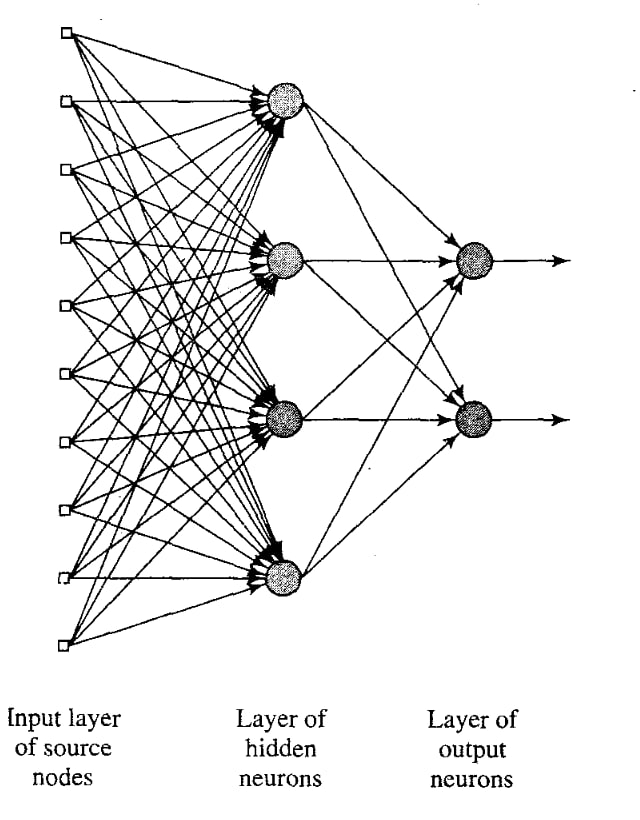
\includegraphics[scale=0.5]{images/MLP}}
\caption{ Ejemplo de ANN con una única capa oculta y con dos salidas. Imagen extraída de \cite{Haykin}.}
\label{fig:red_neuronal_ff}
\end{figure}

Si se considera ahora la función $f$ que implementa un red MLP, se tiene que esta depende de los pesos de la red. Una vez se tengan unos datos con los que entrenar la red y una función de coste que evalúe el rendimiento de la red, se puede aplicar el gradiente descendente estocástico para entrenar la red modificando los pesos de esta. Sin embargo, el cálculo del gradiente de la función de error en un red puede resultar muy costoso, especialmente para el cálculo de las derivadas parciales del error respecto de los pesos de las neuronas en las capas menos profundas. Es por esto que se suele utilizar un algoritmo, denominado \textbf{backpropagation}, para el cálculo del gradiente. 

Este algoritmo está basado en la aplicación de la regla de la cadena que dicta que si se tiene una función $f$ que depende de otra función $g$ que a su vez depende de otra función $h$, entonces se cumple que:
\begin{align*}
\frac{\partial f}{\partial z} = \frac{\partial f}{\partial g} \frac{\partial g}{\partial z}
\end{align*}

De esta forma se puede calcular la parcial de la función de coste respecto a los pesos de una capa utilizando las parciales respecto de los pesos de la siguiente. Luego aplicando esto desde el final al principio de la red, se consigue agilizar el cálculo del gradiente de la función de coste.

\subsection*{Funciones de activación}

Como se comenta en la ecuación \eqref{eq:salida_neurona}, la salida de una neurona es una suma ponderada de las entradas más un sesgo, a las que se le aplica una función de activación. La inclusión de este tipo de funciones es para evitar que la red sea lineal. Si la ecuación \eqref{eq:salida_neurona} fuese idéntica sin aplicar la función de activación entonces la salida de la red sería una función lineal respecto de la entrada, esto es, un polinomio de primer grado. Esto haría que la red no pudiera implementar funciones complejas lo que es necesario para aprender patrones más complejos presentes en los datos.  Es por esto que normalmente las funciones de activación deben ser funciones no lineales. Destacar que la función de activación debe ser derivable para poder calcular el gradiente de la función de coste con el algoritmo \textit{backpropagation} cuando se entrene la red.

Existen varias funciones de activación que se pueden utilizar, sin embargo son especialmente interesantes la función de activación \textbf{ReLU} (\textit{rectifier linear unit}) definida como $ f(x) = max\{0,x\}$ y la \textbf{sigmoidal} definida como $f(x) = \frac{1}{1+e^{-x}}$. Se pueden ver sus gráficas en la figura \ref{fig:ejemplos_activacion_relu} y la figura \ref{fig:ejemplos_activacion_sigmoidal}, respectivamente.

La función de activación ReLU es la que se suele usar en las neuronas de las capas ocultas pues contrarresta el \textbf{problema de desvanecimiento del gradiente}. Un problema que afecta al entrenamiento de las redes neuronales que causa que cuando se calcula el gradiente del error para actualizar los pesos este tome valores muy pequeños haciendo que los pesos de la red cambien muy lentamente. Esto dificulta, o incluso impide, el entrenamiento de la red. Además esta función de activación es la más usada normalmente y tiene mejor rendimiento en la mayoría de los casos.

La función de activación sigmoidal se suele utilizar en la capa de salida en los problemas de clasificación binarios.

\begin{figure}[h]
\noindent
\makebox[\textwidth]{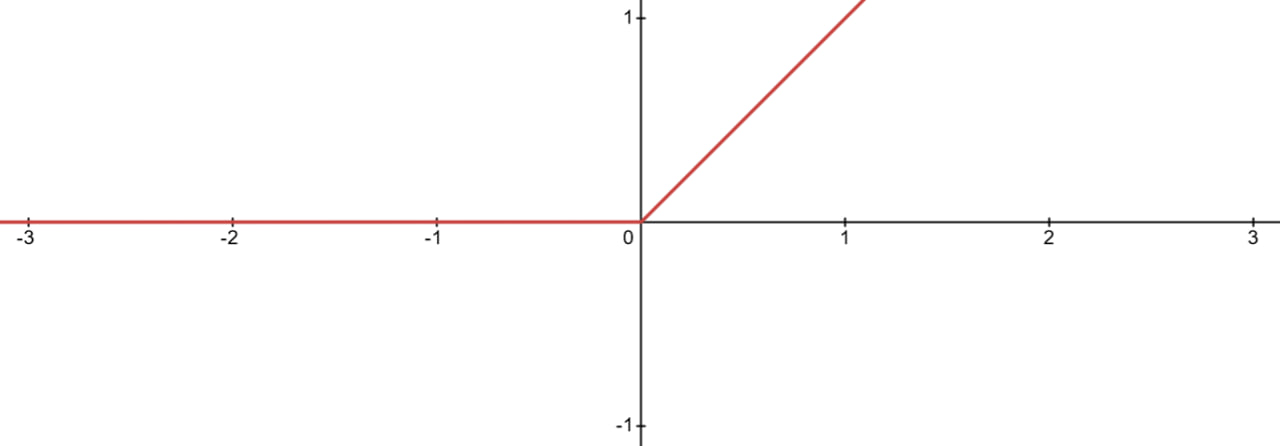
\includegraphics[scale=0.35]{images/relu}}
\caption{Función de activación ReLU.}
\label{fig:ejemplos_activacion_relu}
\end{figure}

\begin{figure}[h]
\noindent
\makebox[\textwidth]{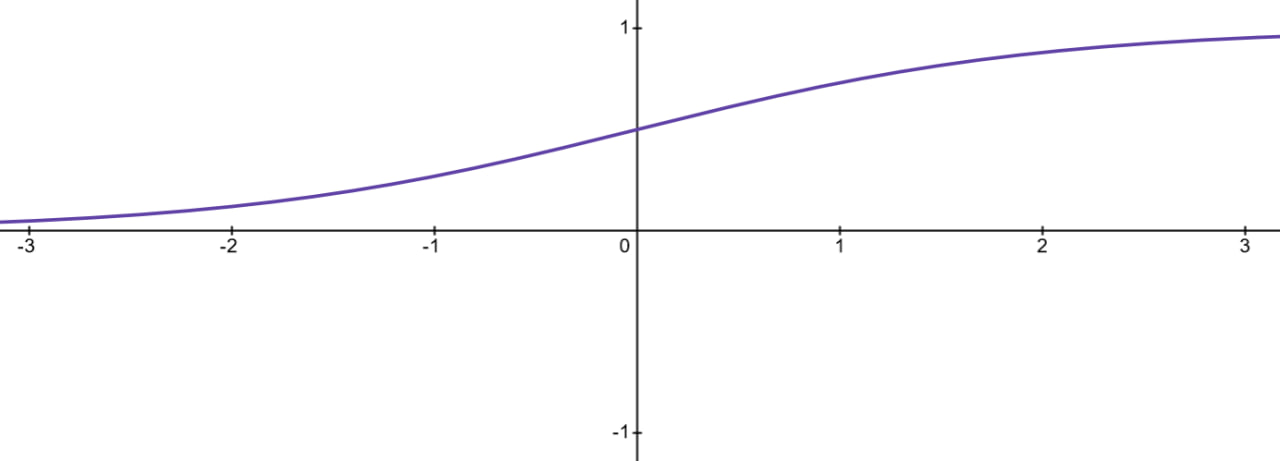
\includegraphics[scale=0.35]{images/sigmoidal}}
\caption{Función de activación sigmoidal.}
\label{fig:ejemplos_activacion_sigmoidal}
\end{figure}



\subsection*{Batch normalization}

\textbf{Batch normalization} \cite{ioffe2015batch} es una método consistente en normalizar los datos de entrada de cada capa. De esta manera se consigue independizar la distribución de los datos de entrada de cada capa de la red, con los parámetros aprendidos por la red. Está probado que este método hace que el entrenamiento de la red sea más estable y más rápido. Además también se sabe que tiene un efecto regularizador en la red, lo que disminuye la probabilidad de que la red sobreentrene.

\subsection*{Dropout}

\textbf{Dropout} \cite{hinton2012improving} se refiere a la técnica utilizada en redes neuronales consistente en ignorar algunas neuronas de forma aleatoria durante el periodo de entrenamiento. Usualmente se le da a cada neurona una probabilidad $p$ de ser ignorado, y en cada paso del algoritmo de entrenamiento se desconecta cada neurona de la red con dicha probabilidad. De esta forma se busca que ninguna neurona sea muy dependiente de la salida de otra neurona específica. Esta técnica regulariza la red lo que hace que la red sea menos propensa a sobreentrenar.

\subsection{Redes convolucionales}
La \textbf{redes convolucionales} (\textit{Convolutional neural networks}, CNN) \cite{9451544} son un tipo de red neuronal feedforward diseñadas para procesar datos en forma de múltiples arrays. En nuestro caso nos centraremos en el caso en el que la entrada son imágenes, que son arrays en 2 dimensiones (matrices) que contienen tres \textbf{canales}, uno por cada color.  La estructura las CNNs es una capa de entrada, seguida de varias capas ocultas y una capa de salida. Las capas ocultas suelen estar compuestas por una o varias \textbf{capas convolucionales} seguidas de una \textbf{capa de pooling}, esto repetido varias veces. Además al final de la red se suelen colocar una o varias \textbf{capas totalmente conectadas} hasta la capa de salida.

\subsection*{Capas convolucionales}
Una \textbf{convolución} es un operador matemático que recibe dos funciones $f,g:\mathbb{R}\rightarrow \mathbb{R}$ y la transforma en otra función $f\ast g$ definida como sigue:
\begin{align*}
(f \ast g)(t) = \int_{-\infty}^{\infty} f(x)g(t-x)dx
\end{align*}
Basado en este operador, existe la \textbf{convolución discreta} en 2 dimensiones, que se define como sigue:

\begin{align*}
(f\star g)[i,j] = \sum_{m=-\infty}^{\infty}\sum_{n=-\infty}^{\infty}f(m,n)g(i-m,j-n)
\end{align*}

Este operador no es más que la adaptación de la convolución al caso en el que $f$ y $g$ sean funciones discretas, es decir, definidas sobre los números enteros, $\mathbb{Z}$. Este es el operador que aplican las capas convolucionales a sus entradas. En el caso de las convoluciones aplicadas en una CNN $f$ se corresponde con la entrada de la capa convolucional y $g$ con el \textbf{núcleo}, \textbf{kernel} o \textbf{filtro}. de la convolución. El \textit{kernel} no es más que una matriz de dimensiones $n\times m$ de valores reales. Véase la Figura \ref{fig:ejemplo_convolucion} para ver un ejemplo de una convolución.

 
\begin{figure}[h]
\noindent
\makebox[\textwidth]{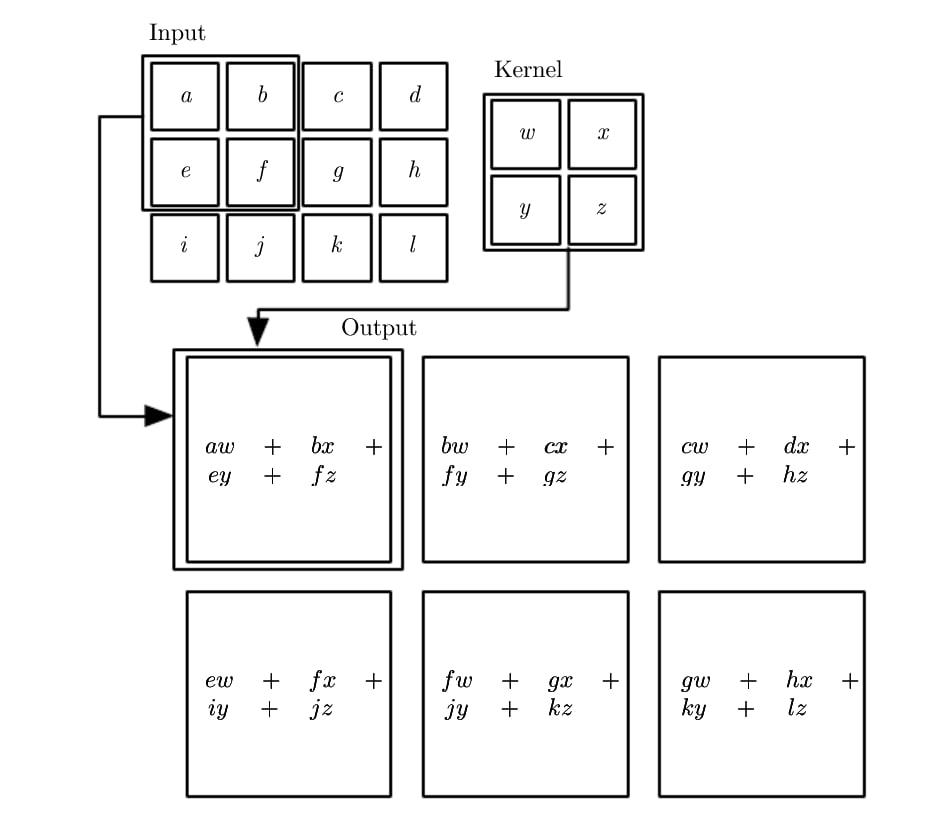
\includegraphics[scale=0.5]{images/ejemplo_convolucion}}
\caption{En esta imagen se puede ver un ejemplo de una convolución aplicada a una entrada de dimensiones $3\times 4$ por un kernel de dimensiones $2\times 2$. Se puede ver que la salida tiene tamaño $2\times 3$. Notablemente se puede ver que al contrario que en la definición de la operación de convolución dada, aquí no se le da la vuelta al kernel, como suele ocurrir en la práctica. Imagen extraída de \cite{Goodfellow-et-al-2016}.}
\label{fig:ejemplo_convolucion}
\end{figure}

Usualmente la entrada de las capas convolucionales tienen más de un canal (por ejemplo la capa inicial suele tener 3 canales, uno por cada color primario), en tal caso, el \textit{kernel} tiene tantos canales como la entrada y aplica cada uno a su canal correspondiente, sumando la salida. Para un ejemplo ver la Figura \ref{fig:ejemplo_convolucion_3canales}. A la salida de una convolución se le llama \textbf{mapa de características}. 

Por lo visto hasta ahora, el filtro se aplica posición a posición de izquierda a derecha y de arriba hacia abajo. Se denomina \textbf{stride} al parámetro que determina cada cuantas posiciones se aplica el filtro. Por ejemplo un stride de 1 aplica el filtro de forma normal. Otro parámetro que se utiliza es el \textbf{padding} que indica si se debe expandir la imagen por los bordes y con qué valores expandirla en caso de hacerlo. Por ejemplo, en la figura \ref{fig:ejemplo_convolucion} no se utiliza \textit{padding} y por lo tanto la salida tiene una fila y una columna menos.

\begin{figure}[h]
\noindent
\makebox[\textwidth]{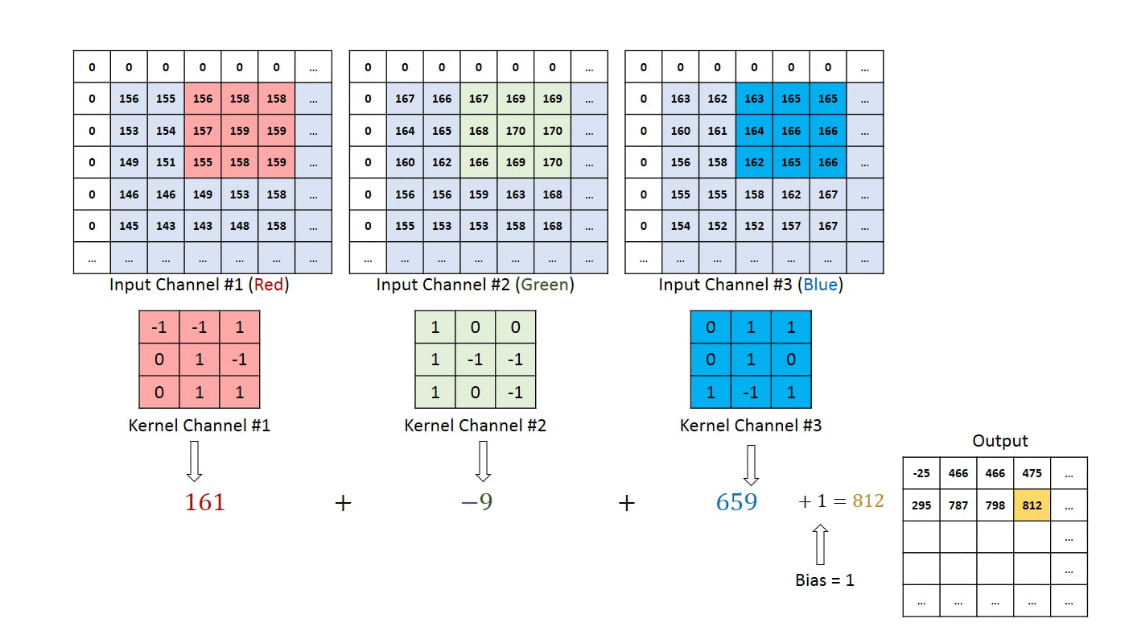
\includegraphics[scale=0.5]{images/ejemplo_convolucion_3canales}}
\caption{Aquí se puede ver un ejemplo de una convolución aplicada a una entrada con 3 canales, uno por cada color primario. Se ve cómo el kernel ahora tiene 3 canales también. Imagen extraída de \url{https://saturncloud.io/blog/a-comprehensive-guide-to-convolutional-neural-networks-the-eli5-way/}.}
\label{fig:ejemplo_convolucion_3canales}
\end{figure}

Ahora que ya está claro qué es una convolución, ya se puede definir una capa convolucional como una capa que aplica $n\in \mathbb{N}$ convoluciones a una entrada. Al número de convoluciones se le denomina \textbf{profundidad} y determina el número de canales que tendrá la salida de la capa. Las dimensiones espaciales de la salida dependerán de las dimensiones espaciales de la entrada y a las decisiones de \textit{padding} y \textit{stride} que se hagan. Además se aplica una función de activación, posición a posición, a la salida de la capa. Esta función habitualmente es la ReLU por las razones que ya se dieron en la subsección de funciones de activación.

El objetivo de las capas convolucionales es la detección de características locales de la entrada de la capa anterior ya que cada convolución aplica la misma operación localmente a lo largo de toda la entrada. Además, este tipo de capas tienen un número reducido de parámetros a aprender por la red ya que sólo hace falta aprender los pesos de los filtros.

\subsection*{Capas de pooling}

Las capas de \textit{pooling} se encargan de reducir las dimensiones espaciales de la entrada manteniendo el número de canales. Esto es, disminuyen el número de filas y columnas. Para ello dividen cada mapa de características en ventanas disjuntas que cubren todas las filas y columnas, y ``\textit{resumen}''  todos los valores en una ventana a uno sólo. Esto disminuye el coste computacional de la red. Este tipo de capas también busca juntar valores que son similares en uno sólo.

Los dos tipo típicos de \textit{pooling} son el \textbf{max pooling} que toma el máximo de los valores de la ventana y el \textbf{average pooling} que toma la media aritmética de los valores de la ventana. Se cree que \textit{max pooling} tiene mejor rendimiento y, de hecho, en la parte matemática de este TFG se pueden ver argumentos de por qué podría ser cierto. En la Figura \ref{fig:ejemplo_pooling} se puede ver un ejemplo de ambos tipos de \textit{pooling}.



\begin{figure}[h]
\noindent
\makebox[\textwidth]{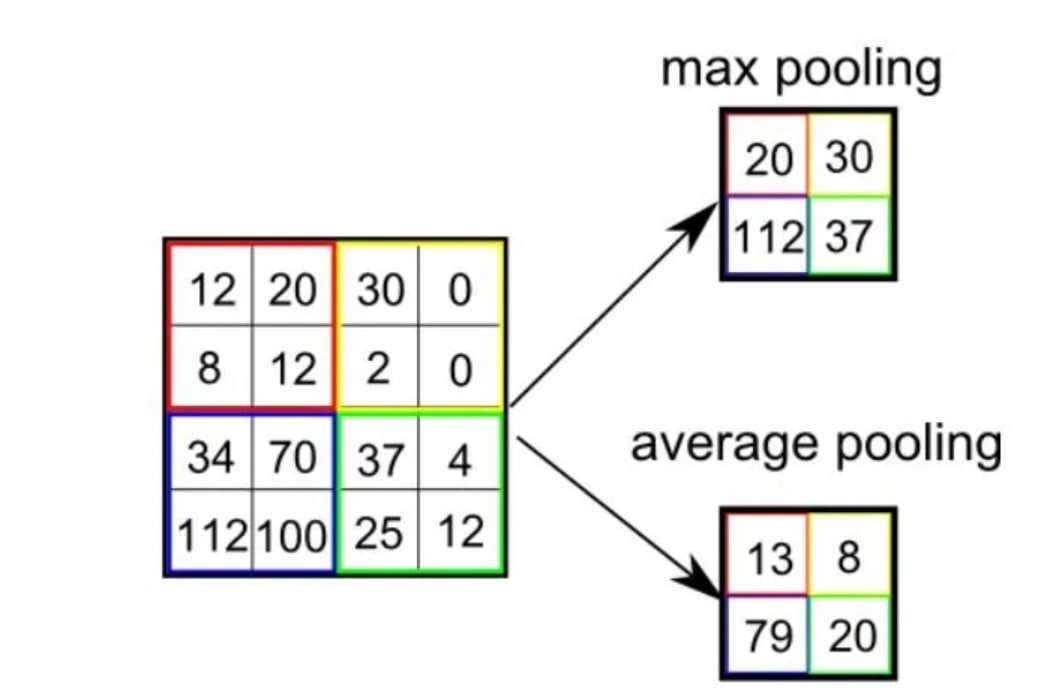
\includegraphics[scale=0.3]{images/ejemplo_pooling}}
\caption{En la figura se ver cómo se aplica \textit{max pooling} y \textit{average pooling} a una entrada. Como las ventanas tienen tamaño $2\times 2$ se dice que se aplica \textit{pooling} $2\times 2$. Imagen extraída de \url{https://saturncloud.io/blog/a-comprehensive-guide-to-convolutional-neural-networks-the-eli5-way/}.}
\label{fig:ejemplo_pooling}
\end{figure}

\subsection*{Capas totalmente conectadas}
Este tipo de capas no son más que una capa típica de MLP que conecta todos los valores de las neuronas de la capa anterior con todas las neuronas de esta capa. Se colocan después de todas las capas convolucionales de \textit{pooling}. Por ejemplo, si se quisiera resolver un problema de clasificación de imágenes en cinco clases, se tendría una última capa totalmente conectada con cinco neuronas.


\section{XAI}

\subsection{LIME}

\subsection{Métricas ReVEL}

\subsection{Regularización X-Shield}


\newpage
\chapter{Estado del arte} \label{cap:eda}


En esta sección hago búsquedas en Scopus para ver el estado del arte y analizarlo. Para seros sinceros no tengo muy claro que debería buscar ya que dudo que encuentre artículos que apliquen explicabilidad a detección de cánceres de próstata (aunque está bien hacer la búsqueda para tenerlo claro). 

Por otro lado quizás debería buscar trabajos que traten la detección automática de cánceres de próstata o que apliquen explicabilidad a otras tareas médicas a ver que encuentro. Estoy interesado en ver cómo debería enfocar el estado del arte.

\newpage
\chapter{Métodos} \label{cap:met}
En este capítulo introduciría qué son las métricas revel en profundidad (cálculo/interpretación) + La regularización X-SHIELD. Luego introduciría mis propuestas. Antes de introducir mis propuestas haría un introducción sobre EfficientNet (en particular efficientnet b2) e introduciría su arquitectura y por qué la he elegido.

\section{Métricas ReVEL} \label{sec:FSCNet} 
\section{X-Shield} 


\clearpage
\section{Métodos propuestos} \label{sec:metodospropuestos}
\subsection{EfficientNet}
\subsection{FXShield}
\subsection{FRShield}
\subsection{HShield}

\clearpage

\section{Implementación}

Aquí explico de qué código he partido (+ GitHub), breve introducción de cómo está organizado el proyecto (en carpetas/archivos), los datos, cómo me he organizado el proyecto en conda (versión de python + modulos) finalmente pondría un link al proyecto en mi GitHub). Por cierto me interesa saber si prefieres que cree un fork de alguno de tus proyectos en github (Iván) o si me creo uno a parte en el mío (obviamente referenciando tu github como partida), a mi me da igual.



\clearpage


\newpage
\chapter{Experimentos} \label{cap:exp}


\section{Datos empleados} \label{sec:datos}
En esta sección explico el conjunto de datos del que parto. Explico como está organizado, cómo están balanceadas las clases, qué clases hay, qué significan, puedo mostrar algunos datos para mostrar ejemplos (si tengo permiso, claro). Me interesa saber de dónde provienen los datos también para ponerlo. En cuanto a estudio cualitativo de estos no creo que yo pueda aportar mucho así que no creo que haga (además de que hay demasiados datos).
\section{Experimentos realizados}

\subsection{Separación de datos}

Cómo están divididos los datos. He utilizado un conjunto de validación ya que validación cruzada es demasiado costoso en tiempo.

\paragraph*{Validation}

\paragraph*{Optimizador y elección de hiperparámetros}



\section{Métricas}
Explico que he utilizado Accurcy, cross entropy error y recuerdo el uso de la métricas revel. También hablo de los test estadísticos que he utilizado y los parámetros escogidos.
\paragraph*{Test estadísticos bayesianos}


\section{Resultados}

Aquí muestro mis resultados + curvas de aprendizaje y comento brevemente estos.

\section{Discusión} \label{sec:discusion}
Aquí es donde discuto mis resultados obtenidos.


\clearpage
\chapter{Conclusiones} \label{cap:conc}
Conclusiones del TFM y si he conseguido los objetivos que me propuse al inicio.

\section{Trabajos futuros}

Aquí comento trabajos futuros. Cómo probar con otros datsets o lo que comentamos de sacar las métricas REVEL sobre features (en nuestra primera charla).


